% Template for PLoS
% Version 3.1 February 2015
%
% To compile to pdf, run:
% latex plos.template
% bibtex plos.template
% latex plos.template
% latex plos.template
% dvipdf plos.template
%
% % % % % % % % % % % % % % % % % % % % % %
%
% -- IMPORTANT NOTE
%
% This template contains comments intended 
% to minimize problems and delays during our production 
% process. Please follow the template instructions
% whenever possible.
%
% % % % % % % % % % % % % % % % % % % % % % % 
%
% Once your paper is accepted for publication, 
% PLEASE REMOVE ALL TRACKED CHANGES in this file and leave only
% the final text of your manuscript.
%
% There are no restrictions on package use within the LaTeX files except that 
% no packages listed in the template may be deleted.
%
% Please do not include colors or graphics in the text.
%
% Please do not create a heading level below \subsection. For 3rd level headings, use \paragraph{}.
%
% % % % % % % % % % % % % % % % % % % % % % %
%
% -- FIGURES AND TABLES
%
% Please include tables/figure captions directly after the paragraph where they are first cited in the text.
%
% DO NOT INCLUDE GRAPHICS IN YOUR MANUSCRIPT
% - Figures should be uploaded separately from your manuscript file. 
% - Figures generated using LaTeX should be extracted and removed from the PDF before submission. 
% - Figures containing multiple panels/subfigures must be combined into one image file before submission.
% For figure citations, please use "Fig." instead of "Figure".
% See http://www.plosone.org/static/figureGuidelines for PLOS figure guidelines.
%
% Tables should be cell-based and may not contain:
% - tabs/spacing/line breaks within cells to alter layout or alignment
% - vertically-merged cells (no tabular environments within tabular environments, do not use \multirow)
% - colors, shading, or graphic objects
% See http://www.plosone.org/static/figureGuidelines#tables for table guidelines.
%
% For tables that exceed the width of the text column, use the adjustwidth environment as illustrated in the example table in text below.
%
% % % % % % % % % % % % % % % % % % % % % % % %
%
% -- EQUATIONS, MATH SYMBOLS, SUBSCRIPTS, AND SUPERSCRIPTS
%
% IMPORTANT
% Below are a few tips to help format your equations and other special characters according to our specifications. For more tips to help reduce the possibility of formatting errors during conversion, please see our LaTeX guidelines at http://www.plosone.org/static/latexGuidelines
%
% Please be sure to include all portions of an equation in the math environment.
%
% Do not include text that is not math in the math environment. For example, CO2 will be CO\textsubscript{2}.
%
% Please add line breaks to long display equations when possible in order to fit size of the column. 
%
% For inline equations, please do not include punctuation (commas, etc) within the math environment unless this is part of the equation.
%
% % % % % % % % % % % % % % % % % % % % % % % % 
%
% Please contact latex@plos.org with any questions.
%
% % % % % % % % % % % % % % % % % % % % % % % %

\documentclass[10pt,letterpaper]{article}
\usepackage[top=0.85in,left=2.75in,footskip=0.75in]{geometry}
%Brian's additions:
\usepackage{booktabs}  
% Use adjustwidth environment to exceed column width (see example table in text)
\usepackage{changepage}

% Use Unicode characters when possible
\usepackage[utf8]{inputenc}

% textcomp package and marvosym package for additional characters
\usepackage{textcomp,marvosym}

% fixltx2e package for \textsubscript
\usepackage{fixltx2e}

% amsmath and amssymb packages, useful for mathematical formulas and symbols
\usepackage{amsmath,amssymb}

% cite package, to clean up citations in the main text. Do not remove.
\usepackage{cite}

% Use nameref to cite supporting information files (see Supporting Information section for more info)
\usepackage{nameref,hyperref}

% line numbers
\usepackage[right]{lineno}

% ligatures disabled
\usepackage{microtype}
\DisableLigatures[f]{encoding = *, family = * }

% rotating package for sideways tables
\usepackage{rotating}

% Remove comment for double spacing
%\usepackage{setspace} 
%\doublespacing

% Text layout
\raggedright
\setlength{\parindent}{0.5cm}
\textwidth 5.25in 
\textheight 8.75in

% Bold the 'Figure #' in the caption and separate it from the title/caption with a period
% Captions will be left justified
\usepackage[aboveskip=1pt,labelfont=bf,labelsep=period,justification=raggedright,singlelinecheck=off]{caption}

% Use the PLoS provided BiBTeX style
\bibliographystyle{plos2015}

% Remove brackets from numbering in List of References
\makeatletter
\renewcommand{\@biblabel}[1]{\quad#1.}
\makeatother

% Leave date blank
\date{}

% Header and Footer with logo
\usepackage{lastpage,fancyhdr,graphicx}
\usepackage{epstopdf}
\pagestyle{myheadings}
\pagestyle{fancy}
\fancyhf{}
\lhead{\includegraphics[width=2.0in]{PLOS-submission.eps}}
\rfoot{\thepage/\pageref{LastPage}}
\renewcommand{\footrule}{\hrule height 2pt \vspace{2mm}}
\fancyheadoffset[L]{2.25in}
\fancyfootoffset[L]{2.25in}
\lfoot{\sf PLOS}

%% Include all macros below

\newcommand{\lorem}{{\bf LOREM}}
\newcommand{\ipsum}{{\bf IPSUM}}

%% END MACROS SECTION


\begin{document}
\vspace*{0.35in}

% Title must be 250 characters or less.
% Please capitalize all terms in the title except conjunctions, prepositions, and articles.
\begin{flushleft}
{\Large
\textbf\newline{A cost-agnostic probabilistic characterization of the high-dimensional structure of feasible motor commands}
}
\newline
\\
Brian A. Cohn\textsuperscript{1,\Yinyang},
May Szedl\'{a}k \textsuperscript{2,\Yinyang},
Komei Fukuda\textsuperscript{2,\ddag},
Bernd G{\"a}rtner \textsuperscript{2,\ddag},
Francisco J. Valero-Cuevas\textsuperscript{1*,\ddag}
\\
\bigskip
\bf{1} University of Southern California, Department of Biomedical Engineering, Los Angeles, CA, USA
\\
\bf{3} Swiss Federal Institute of Technology, Department of Theoretical Computer Science, Zurich, Switzerland 
\bigskip

% Insert additional author notes using the symbols described below. Insert symbol callouts after author names as necessary.
% 
% Remove or comment out the author notes below if they aren't used.
%
% Primary Equal Contribution Note
\Yinyang These authors contributed equally to this work.

% Additional Equal Contribution Note
% Also use this double-dagger symbol for special authorship notes, such as senior authorship.
\ddag These authors also contributed equally to this work.

% Current address notes
\textcurrency Ronald Tutor Hall, RTH-404 
3710 S. McClintock Ave 
Los Angeles, CA 90089-2905, USA  
% Group/Consortium Author Note
%\textpilcrow Membership list can be found in the Acknowledgments section.

% Use the asterisk to denote corresponding authorship and provide email address in note below.
* valero@usc.edu

\end{flushleft}
% Please keep the abstract below 300 words
\section*{Abstract}
\begin{abstract}
The brain must select its control strategies among an infinite set of possibilties, thereby solving an optimization problem. 
While this set is infinite and lies in high dimensions, it is bounded by kinematic, neuromuscular, and anatomical constraints, within which the brain must select optimal solutions. 
We use data from a human index finger with 7 muscles, 4DOF, and 4 output dimensions. For a given force vector at the endpoint, the feasible activation space is a 3D convex polytope, embedded in the 7D unit cube.
It is known that explicitly computing the volume of this polytope can become too computationally complex in many instances. 
We generated random points in the feasible activation space using the Hit-and-Run method, which converged to the uniform distribution. 
After generating enough points, we computed the distribution of activation across each muscle, shedding light onto the structure of these solution spaces- rather than simply exploring their maximal and nimimal values. 
We also visualize the change in these activation distributions as we march toward maximal feasible force production in a given direction. 
Using the parallel coordintes method, we visualize the connection between the muscle activations. Once can then explore the feasible activation space, while constraining certain muscles.
Although this paper presents a 7 dimensional case of the index finger, our methods extend to systems with up to at least 40 muscles. We challenge the community to map the shapes distributions of each variable in the solution space, thereby providing important contextual information into optimization of motor cortical function in future research.
\end{abstract}
% Please keep the Author Summary between 150 and 200 words
% Use first person. PLOS ONE authors please skip this step. 
% Author Summary not valid for PLOS ONE submissions.   
\section*{Author Summary}

\section{Author Summary}
brian is a phd student\\
may is a phd student\\
bernt, komei, and francisco are professors
\linenumbers

\section*{Introduction}

\section{INTRODUCTION}

Muscle redundancy is the term used to describe the underdetermined nature of neural control of musculature.
The classical notion of muscle redundancy  proposes that, faced with an infinite number of possible muscle activation patterns for a given task, the nervous system uses optimization to select a given specific solution.
Here, each of the $N$ muscles represents a dimension of control, and a muscle activation pattern is a point in $\mathbb{R}^N$ \cite{Valero-Cuevas1998Large}.
Thus researchers often seek to infer the optimization approach and the cost functions the nervous system likely utilizes to find the points in activation space to produce natural behavior \cite{Chao1978Graphical,Prilutsky2000Muscle,scott2004optimal,todorov2002optimal,crowninshield1981physiologically,higginson2005simulated}. 


Implicit in these optimization procedures is the notion that there exists a well structured set of feasible solutions. Thus several of us have focused on describing and understanding those high-dimensional subspaces  embedded in $\mathbb{R}^N$ \cite{kutch2011muscle,kutch2012challenges,sohn2013cat_bounding_box,Valero-Cuevas1998Large,Valero-Cuevas2015high-dimensional}.

For the case of muscle redundancy for submaximal and static force production with a limb,  the problem is phrased as one of computational geometry: find the convex polytope of feasible muscle activations given the mechanics of the limb and the constrains of the task \cite{avis1992Pivoting,Valero-Cuevas1998Large,Valero-Cuevas2009mathematical,Valero-Cuevas2015high-dimensional}.  This convex polytope is called the \emph{feasible activation set}. To date, the structure of this high-dimensional polytope is inferred by its bounding box  \cite{kutch2011muscle,sohn2013cat_bounding_box,Valero-Cuevas2015high-dimensional}.  But the bounding box of a convex polytope will always overestimate its volume, and lose the details of its shape.  Empirical dimensionality-reduction methods have also been used to calculate a basis vectors for such subspaces \cite{Clewley2008Estimating,davella2005shared,krishnamoorthy2003muscle}. But those basis  vectors only provide a description of the dimension, orientation, and aspect ratio of the polytope, but not of its boundaries or internal  structure.

Here we present a novel application of the well-known Hit-and-Run algorithm \cite{smith1984efficient} to describe the internal structure of these high-dimensional feasible activation sets. We apply our technique to a schematic example with three muscles to describe the method, and then use realistic model of an index finger with seven muscles and four joints \cite{Valero-Cuevas1998Large}.
% You may title this section "Methods" or "Models". 
% "Models" is not a valid title for PLoS ONE authors. However, PLoS ONE
% authors may use "Analysis" 
\section*{Methods}
\section{METHODS}
In the case of a tendon-driven limb with $n$ muscles, the feasible activation space is the unit $n$-hypercube (as muscles can only be activated positively from 0 to a maximal normalized value of 1). As explained in \cite{Valero-Cuevas2009mathematical}, when task constraints are introduced to the system, the feasible activation set is further reduced; in this context, a task is a static force vector produced at the endpoint of the limb, which is represented as a set of inequality and equality constraints. Thus if this simple limb meets all constraints, the feasible activation set of the polytope $P$ contains all feasible activations  $\textbf{a} \in \mathbb{R}^n$ that satisfy
\[\textbf{f} = A\textbf{a}, \textbf{a} \in [0,1]^n,\]
where $\textbf{f} \in \mathbb{R}^m$ is a fixed force vector and $A = J^{-T}RF_o \in \mathbb{R}^{m \times n}$--- where $J$, $R$ and $F_0$ are the matrices of the Jacobian of the limb, the moment arms of the tendons, and the strengths of the muscles, respectively \cite{Valero-Cuevas1998Large,Valero-Cuevas2009mathematical}. $P$ is bounded by the unit $n$-cube since all variables $a_i$, $i \in [n]$ are bounded by 0 and 1 from below, above respectively.
Consider the following $1 \times 3$ fabricated example, where the task is a 1N unidimensional force.
\begin{align*}
&1 = \frac{10}{3}a_1 - \frac{53}{15}a_2 + 2a_3 \\
&a_1, a_2, a_3 \in [0,1],
\end{align*}



\begin{figure}[schematic_arm]
  \label{fig:schematic_arm}
  \centering
  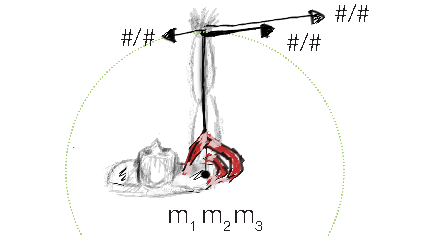
\includegraphics[width=0.5\textwidth]{sections/figs/schematic_example_drawing.pdf}
  \caption{One imagined visualization of the fabricated tendon driven system, with 3 generators.}
  \label{fig:finger}
\end{figure}


the set of feasible activations is given by the shaded set in Figure \ref{fig:fig_hr}.

\begin{figure}[ht]
  \label{fig:fig_hr}
   \begin{center}
    \includegraphics[width=0.25\textwidth]{sections/figs/feasibleactivation.png}
  \end{center}
  \caption{The feasible activation set for a  three-muscle system meeting one functional constraint is a polygon in $\mathbb{R}^3$. Note that muscle activations are assumed to be bounded between $0$ and $1$.}

\end{figure}

\subsection{Hit-and-Run algorithm}
Hit-and-Run is a method used to uniformly sample a convex body \cite{smith1984efficient}. The mixing time is known to be $\mathcal{O}^*(n^2R^2/r^2)$, where $R$ and $r$ are the radii of the inscribed and cicumscribed ball of $K$ respectively \cite{Dyer, Lovasz}. I.e., after $\mathcal{O}^*(n^2R^2/r^2)$ steps of the Hit-and-Run algorithm has sampled a point uniformly at random (u.a.r.\ ) in the convex body. Unfortunately the hidden constant is large, which makes the problem practically almost infeasible. However experimental results suggest that a number of points linear w.r.t.\ to the dimension suffices, which will be discussed in Section \ref{sec_lengthrun}. 
As the feasible activation space of the muscles are given by a convex polytope, this method can be directly used for our problem.
%Hit-and-Run is a method used to uniformly sample a convex body \cite{smith1984efficient}. As the set of all feasible activations is defined by the mechanics of the limb and the constraints of the task (described in \ref{ss:finger}), we decided to use Hit-and-run to sample muscle activation solutions from the polytope $P$. We refer to each sample from $P$ as a 'point' $p \in [0,1]^n$.

The Hit-and-Run walk on $P$ is defined as follows (it works analogously for any convex body):
\begin{enumerate}
\item Find a starting point $\textbf{p}$ of $P$ %(Figure \ref{fig:hitruncube}a) .
\item Generate a random direction from $\textbf{p}$ in $P$ (uniformly at random over all directions) (Figure \ref{fig:hitruncube}a).
\item Find the intersection points of the random direction with the edges of the polytope (Figure \ref{fig:hitruncube}b).
\item Choose a point u.a.r.\ on this line segment given by the intersection points (Figure \ref{fig:hitruncube}c). 
\item Repeat from $1.$ the above steps with the new point as the starting point .
\end{enumerate}

\begin{figure}[htbp]
\centering
\includegraphics[width=0.5\textwidth,page=10]{sections/figs/HitandRunSchematics_all.pdf}
\caption{Graphical description of the Hit-and-Run algorithm.}
\label{fig:hitruncube}
\end{figure}

\begin{figure}[htbp]
\centering
\includegraphics[width=0.5\textwidth,page=7]{sections/figs/HitandRunSchematics_all.pdf}
\caption{Distribution of feasible activations for [briantodo: select task percent]50\% maximal force output in the palmar direction.}
\label{fig:prebasis_cube}
\end{figure}

\begin{figure}[htbp]
\centering
\includegraphics[width=0.5\textwidth,page=8]{sections/figs/HitandRunSchematics_all.pdf}
\caption{This shows how the basis vectors are orthogonal following Gram-Schmidt orthogonalization.}
\label{fig:postbasis_cube}
\end{figure}

\begin{figure}[htbp]
\centering
\includegraphics[width=0.5\textwidth,page=9]{sections/figs/HitandRunSchematics_all.pdf}
\caption{Uniform distribution aross the feasible activation space. In the schematic arm example, the distribution is represented within a 2D plane.}
\label{fig:posthitrun_distribution}
\end{figure}



\subsection{Selecting a central seed point}
To find a starting point in 
\[\textbf{f} = A\textbf{a}, \textbf{a} \in [0,1]^n,\]
we only need to find a feasible activation vector. For the Hit-and-Run algorithm to mix faster we want the starting point not close to a corner. %centrally located point within the polytope- that way, the early points will not be clustered in a corner [maytodo cite]. 
We use the following standard trick with slack variables $\epsilon_i$, which for applications often gives a good starting point.% to select a point where activations $a_i$ for all muscles are far from 0 and 1, thereby finding a solution central within $P$ [maytodo cite the use of slack variables to improve mixing time].

\begin{equation}\label{eq:LP_r}
\begin{array}{lrcl}
\mbox{maximize} & \sum_{i=1}^n \epsilon_i \\ 
\mbox{subject to} & \textbf{f} &=& A\textbf{a}\\
  & a_i &\in& [\epsilon_i, 1- \epsilon_i], \hspace{5mm} \forall i \in \{1,\dots,n\}  \\
  & \epsilon_i &\geq& 0, \hspace{5mm} \forall i \in \{1,\dots,n\}.  
\end{array}
\end{equation}

%\subsection{Removing inter-point dependence}
%\label{sec_lengthrun}
%As the function is recursive, any two successive points are not independent; therefore, we sample from our walk on $P$ by selecting every $m^{th}$ point to extract points which are distributed %uniformly-at-random across $P$, and are independent to eachother.
%Some have said that it takes X Hit-and-Run steps before the first and last points gathered are independent of one another, so we chose to collect every [maytodo confirm 100th] point into an array of points %$M = [p_0, p_1, p_2, ... p_{100,000}]$. 



\subsection{Length of Hit-and-Run walk}
\label{sec_lengthrun}
How many points do we need to record from Hit-and-Run to reach a representative distribution across the polytope? For convex polygons in higher dimensions up to $40$, experimental results suggest that $\mathcal{O}(n)$ steps of the Hit-and-Run algorithm are sufficient.
In particular Emiris and Fisikopoulos paper suggest that $(10 + \frac{10}{n})n$ steps are enough to converge upon the uniform distribution \cite{emiris2013efficient}, while in Ge et al.'s paper every point of the Hit-and-Run algorithm is used in the sample \cite{Ge}. 
%With the index finger model we collected a sample of [briantodo number] points.


\subsection{Realistic index finger model}
\label{ss:finger}
We used our published model in \cite{Valero-Cuevas1998Large} to find matrix $A \in \mathbb{R}^{4 \times 7}$, where $\textbf{a} \in \mathbb{R}^7$; the four degrees of freedom were ad-abduction, flexion-extension at the metacarpophalangeal joint, and flexion-extension at the proximal and distal interphalangeal joints.
The force directions we simulated are visible in Figure \ref{fig:finger}. In this model, for each input we collected 1.000.000 points and sampled every 100th point.

\begin{figure}[htbp]
  \centering
  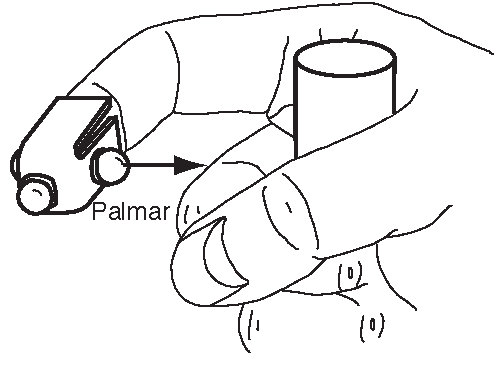
\includegraphics[width=0.5\textwidth]{sections/figs/finger.pdf}
  \caption{The index finger model simulated 50\% of maximal force production in the palmar direction. Adapted from \cite{Valero-Cuevas1998Large}.}
  \label{fig:finger}
\end{figure}



\subsection{Solution projection histograms}
The visualization for the distribution of solutions over each muscles is given in the histogramms \ref{fig:raw_histograms}. Since the generated points are uniformly at random distributed, this gives a close approximation. %The resulting array of points $M$ can be thought of as a matrix, where each row is a point, and each column is a muscle's activation. With this, we can enter a column of this data into a histogram; importantly, this approach projects the density of points. This can be used to approximate the relative volume of different sections of $P$- by slicing (binning) from each muscle's dimension.

\begin{figure}[htbp]
\centering
\includegraphics[width=0.5\textwidth]{sections/figs/raw_histograms.png}
\caption{Distribution of feasible activations for [briantodo: select task percent]50\% maximal force output in the palmar direction.}
\label{fig:raw_histograms}
\end{figure}

\subsection{Parallel coordinates visualization}
A common way to visualize higher dimensional data is using parallel coordinates[briantodo citations]. To show our sample set of points in the feasible activation space we draw $n$ parallel lines for each of the $n$ muscles. With the axis labels of the line set between 0 and 1, each point is then represented by connecting their coordinates by $n-1$ lines. Using an interactive surface we restrict each muscle function to any desired interval- see, figures [maytodo link these to result figures].

\subsection{Muscle-metabolic and neural drive cost functions}

For every solution collected, we used popularly-used cost functions: we computed activation $l_1$, $l_2$ and $l_3$ norms, and the tendon-force $l_1^w$, $l_2^w$ and $l_3^w$ norms. Six additional vertical lines were added to the parallel coordinates plot to represent each cost function. With the same parallel coordinates framework as developed with muscle activation, we can restrict and subset solutions which fall into desired cost-function ranges, thereby masking sub-optimal solutions and highlighting only those meeting the criteria.

\begin{table}[h]
\centering
\begin{tabular}{@{}ll@{}}
\toprule
\textbf{Name} & \textbf{Cost function}  \\ \midrule
$l_1$            & $\sum_{i=1}^n a_i$                                     \\
$l_2$            & $\sqrt{\sum_{i=1}^n a_i^2}$                                    \\
$l_3$            & $\sqrt[3]{\sum_{i=1}^n a_i^3}$                                   \\
$l_1^w$            & $\sum_{i=1}^n a_i F_{0i}$                                    \\
$l_2^w$            & $\sqrt{\sum_{i=1}^n (a_i F_{0i})^2}$                                  \\
$l_3^w$            & $\sqrt[3]{\sum_{i=1}^n (a_i F_{0i})^3}$                                    \\ \bottomrule
\end{tabular}

\caption{Cost functions and their usage, where $a_i$ and $F_{0i}$ represent a muscle's activation in a given solution and that muscles MIC, respectively.}
\label{cost_function_tabls}

\end{table}

For a given point $\textbf{a} \in \mathbb{R}^n$ we are interested in the associated cost of every solution collected through Hit and Run.

We developed and tested our code in  Ubuntu 14.04, Windows 8.1, and OSX Yosemite, using Scala 2.11.6 [briantodo cite] for our implementation of Hit-and-Run, R 3.1.3 [briantodo cite] for histograms and plots, and using Sygmatic Parcoord[briantodo cite] and d3.js[briantodo cite] for our interactive parallel coordinate visualization. All code required to replicate our research is readily available at https://github.com/bcohn12/space.

% Results and Discussion can be combined.
\section*{Results}
We found the feasible activation set for the task of producing nine different sub-maximal magnitudes of static fingertip force in the distal direction, evenly spaced between  $10\%$ and $90\%$ of maximal static force. These are labeled as intensity values $\alpha = 0.1, 0.2., \hdots, 0.9$ in the Figs.  For each sub-maximal force magnitude, we ran 1,000,000 Hit-and-Run iterations and sampled every $100^{th}$ point to produce 10,000 uncorrelated points uniformly distributed in $P$. Recall that for $100\%$ of maximal force $P$ shrinks to a single, unique solution \cite{valero-cuevas2007large}.

\subsection*{Muscle activation histograms}

The histograms in Fig. \ref{fig:raw_histograms} represent the sampled probability distribution of activation for each muscle for the case where the desired fingertip force magnitude in the distal direction is  set to be $\alpha = 0.5$ (i.e., 50% of the maximal possible). 

Fig. \ref{sub:activation_spaces_for_increasing_force} in turn shows  the histograms  all muscles at all nine levels of $\alpha = 0.1$ to $\alpha = 0.9$, as well as the unique solution associated with $\alpha = 1.0$, the  maximal possible  fingertip force in the distal direction. Note that  all histograms include dotted lines indicating the lower- and upper-bounds of sampled activation for each muscle. 

We  validate the Hit-and-Run algorithm by using vertex enumeration methods as in \cite{Valero-Cuevas1998Large,Valero-Cuevas2000Predictive} to find the exact maximal and minimal activation for each muscle (i.e., the individual sides of the bounding box of $P$) at each sub-maximal force level, Figs. \ref{fig:raw_histograms} and \ref{fig:Z_progression}. We found that the difference between the exact and sampled bounds for all muscles was smaller than 0.001, or $<$ 0.1~\% of the $[0, 1]$ range of each muscle. 

\begin{figure}[h]
\centering
\includegraphics[width=0.5\textwidth]{figs/raw_histograms.pdf}
\caption{Distribution of feasible activations for $\alpha= 0.5$ (50\% of the computed maximal force output in the distal direction). Dashed lines are the observed lower and upper bounds.}
\label{fig:raw_histograms}
\end{figure}



\subsection*{Parallel Coordinates Visualization}
While histograms provide detailed descriptions of the relative density of solutions at various levels of activation for each muscle,  parallel coordinates visualization  effectively shows the relatedness of activation levels across muscles for a given task, magnitude of desired fingertip force, and cost.

We applied parallel coordinate visualization to the 10,000 sampled points for each sub-maximal force level to view how different parts of one muscle's distribution interact with the others.
To maintain real-time interactivity of the plot in our interface, and without perceptible loss of accuracy, we used only the first 1,000 points collected for each task, from $\alpha = 0.1$ to $\alpha = 1.0$. This interactive plot can be seen at \texttt{http://parcoords.divshot.io/examples/slickgrid.html}. Fig. \ref{fig:parcoord_full} shows the parallel coordinate visualization for the same case as in Fig. \ref{fig:raw_histograms}.

\begin{figure}[htbp]
\centering
\includegraphics[width=\textwidth]{figs/parcoord_alpha50.pdf}
\caption{This figure is a snapshot of the interactive platform for visualizing 1000 solutions, all of which produce the same static output force in the distal direction.
This parallel coordinates plot visualizes where each feasible activation set is strewn across each dimension's axis as a line. 
While the activation level $\alpha$ could be set to view all tasks, we set $\alpha$ to a distal force of 50\% of the computed maximal feasible force in this direction. 
Here we show 1,000 points accrued from Hit-and-Run on a task of $\alpha=0.5$.}
\label{fig:parcoord_full}
\end{figure}

Parallel coordinates allow us to visualize not only the proportion of solutions lost when limiting one or more muscle activation or cost function to a given range, but also the location and interrelatedness of the remaining solutions. The density of different solutions is additionally highlighted by the color density resulting from  overlapping  lines. While we invite you to explore the nature of the feasible activation set at the interactive website for yourself, Fig. \ref{fig:parcoords} shows six such explorations.

\begin{figure}[htbp]
\centering
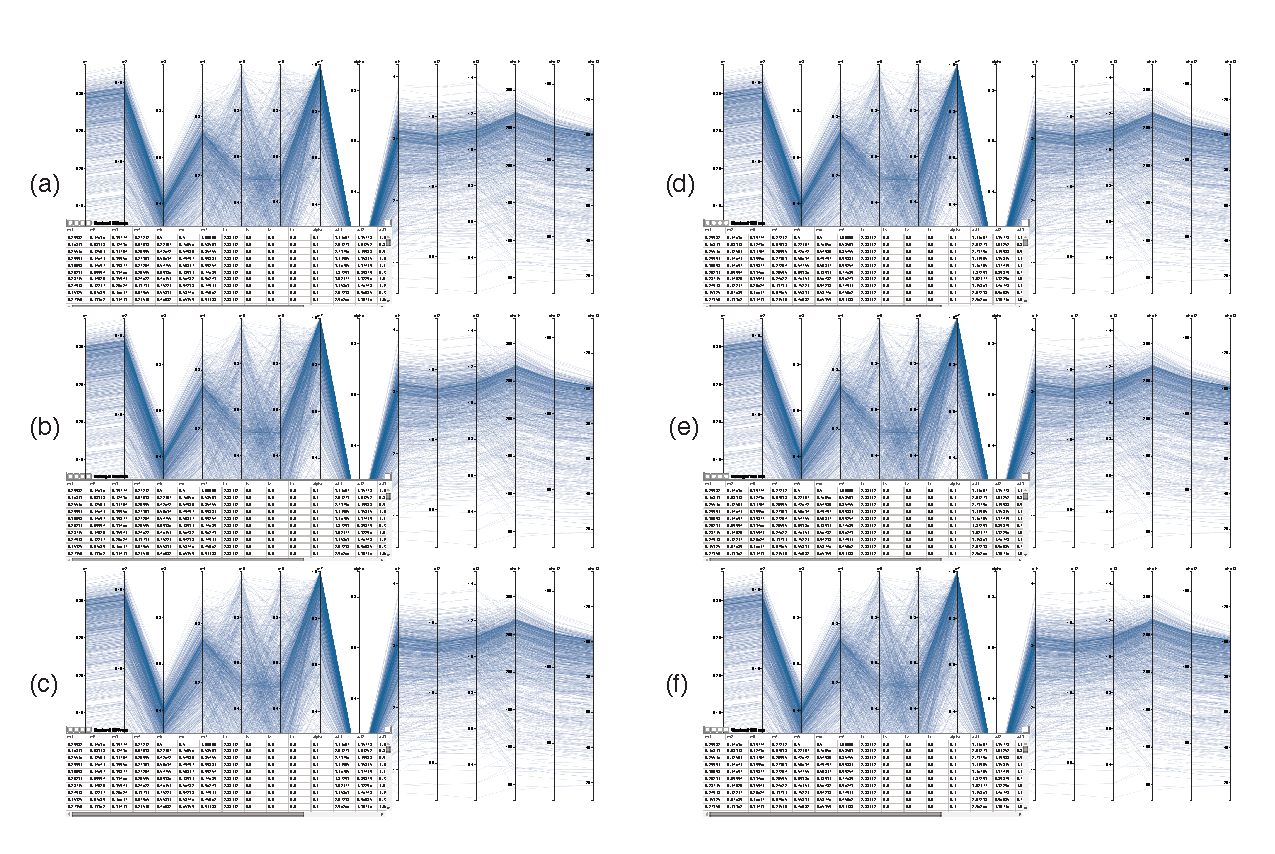
\includegraphics[width=\textwidth]{figs/parcoords.pdf}
\caption{These snapshots show the use of the interactive parallel coordinate visualization of solutions across the activation space. For the task set to 50\% of maximal in the distal direction, we show the
(a) remaining 166 solutions when PI $<$ 60\% 
(b) remaining 57 solutions when DI $<$ 60\%, and the
(c) remaining 57 solutions when we constrain PI $<$ 60\% and DI $<$ 60\%. We also show the
(d) remaining 502 solutions when we select the lower 50\% of $L_1$ costs,
(e) remaining 498 solutions when we select the lower 50\% of $L_2^w$ costs, and the
(f) remaining 220 solutions when we select the lower 50\% across all cost functions in Table \ref{cost_function_tabls} }
\label{fig:parcoords}
\end{figure}

Constraining PI $<$ 60\% still leaves a solution space about three times as large as di $<$ 60\%. 
Observe that constraining DI $<$ 60\% already implies that PI $<$ 60\% as seen in Fig. \ref{fig:parcoords} (b), (c). 
Constraining one muscles does have different effects on the other muscles as for example if ei is constrained below 60\% activation, we see that the bounding box of PI is significantly restricted; however, the same constraint has no effect on the bounding box of EIP.

As there are few steep crossings between $L_1$, $L_2$ and $L_3$, the parallel coordinates suggest correlation of those three cost functions.
Similar correlation is observed for the respective weighted functions.
We provide a scatter plot for their relationships in Appendix Fig. \ref{fig:unweighted_cost_functions} and \ref{fig:weighted_cost_functions}.

% subsection paralleL_coordinates (end)



\subsection*{Changes in the structure of the feasible activation space with increasing force mangitude, a.k.a. how muscle redundancy is lost} % (fold)
\label{sub:activation_spaces_for_increasing_force}
The maximal static fingertip force into any direction (i.e., at $\alpha=1$) is produced by  a unique combination of muscle activations \cite{spoor1983balancing,Chao1978Graphical,valero-cuevas2015fundamentals}. Therefore, the histograms in Fig. \ref{fig:Z_progression} show how the multiple solutions available for sub-maximal forces change and shrink  for increasing force magnitude, from $\alpha=0.1$  to $\alpha=1$. You can track the change in the feasible distributions of a given muscle's activations by following its column from top to bottom ending, naturally, with the unique value needed for maximal force magnitude. 

\begin{figure}[htbp]
\centering
\includegraphics[width=\textwidth]{figs/Z_alphaProgression1430924065026.pdf}
\caption{Distribution of activations in the distal direction and changing force. Each row of histograms uses a Hit-and-Run set. The height of each bar visualizes the percentage of 10,000 solutions found within a given bins that are 0.02 wide (i.e., 2\% of total activation range $[0,1]$).  The shape is as meaningful than the height of individual bins of the histograms. Of note is that the mode of the sub-maximal histograms changes, and is seldom the equivalent of the unique activation value needed to achieve maximal force. The lower- and upper-bounds of the histograms are shown as  vertical dotted lines. [what is that other vertical lines]. To our knowledge this is the first time that the internal structure of the feasible activation set has been visualized.}
\label{fig:Z_progression}
\end{figure}

The solution polytope converges as the difficulty of the task increases; the rate of convergence is different across muscles.
For some muscles the convergence only occurs after $\alpha=0.6$ or $\alpha=0.8$ (as in LUM and EIP), while others converge across the entire progression (e.g.\ DI and PI).
Whereas for example FDS already has a small range of feasible activations at $\alpha=0.1$, EIP has feasible activation $[0,1]$ up to 80\%.

It is imperative to keep in mind that every histogram (regardless of its convergence) is composed of the distribution of all 10,000 points; when the distribution is compressed, the relative percentage of the bars will increase (as evident by the increasing y-axis limits), as we fixed break width ($\Delta x$) to remain constant to 2\% of maximal activation \cite{ball1997elementary}.

The peaks seen in these figures is the perpendicular slice that has the largest relative volume; within the same muscle it does not have to be symmetric between the bounds, and can shift over differing tasks.
As expected, the unique solution at $\alpha=1.0$ appears as a single peak representing 100\% of the sampled points; the bounds and the muscle's unique activation are superimposed.

The most simple finding is that the distributions cannot be inferred by their bounding boxes alone.
Consider the activation distributions between $\alpha = 0.7$ and $\alpha = 0.8$ for LUM, where the median changed by less than 4\% while the lower bound increased by nearly 13\%.
Notably, we observe that a meaningful cross-muscle comparison of point distributions cannot be ascertained by the bounding box. For example, at a task of 10\% of maximal distal force production, EIP and EDC both have lower and upper bounds of 0, and 1, respectively, yet their distributions are thoroughly distinct; the shape of EIP is more symmetric (lower 25\% = 0.36, median = 0.5029, upper 75\% = 0.62), while 75\% of the solutions sampled have EDC higher than 0.74 (see Fig. \ref{fig:Z_progression}).

We find this holds not only for inter-muscle distribution comparisons, but intra-muscular distributions. Consider the significant change in the shape of the distributions across the progression for EDC until the 60\% task; the lower and upper bounds change less than 1\% and 4\%, respectively, while the median shifted by nearly 40\%.
In the most extreme case, the median activation can be exceptionally narrow, while the bounds are wide- for example, EIP at a 90\% task; although activation is bounded between 0.1 and 0.81, approximately 79\% of the solutions exist with EIP activation between just 0.49 and 0.51.

Next, we see that if one muscle had to be fixed throughout the entire force progression, DI and PI would fail; their bounding boxes of tasks below $\alpha=0.4$ do not include the unique solution at $\alpha=1.0$.
We also placed a vertical grey line for the scaled unique solution at maximal force, denoted $\textbf{a}^*$, (e.g. LUM converges to an activation of 1 at maximal distal force, so we put a grey line at 0.8 for $\alpha=0.8$ of maximal distal force).
Since $\alpha \textbf{f}_{\max} = \alpha A \textbf{a}^*$, $\alpha \textbf{a}^*$ is a solution of the feasible activation set at $\alpha$-fraction of the maximal force.
However we observe that for some muscles, these points can lie arbitrarily in the distribution i.e.\ do not have to lie close to the corresponding peaks (e.g.\ musle DI and EIP).





\section*{Discussion}
\section{Discussion}
Mostly to be written by Brian
\subsection{Running Time}
The step of the algorithm which are time consuming are finding a starting point, which solves a linear program and can take exponential running time in worst case. For each fixed force vector we only have to find a starting point and an orthonormal basis once, and are hence not of concern for the running time.

Running one loop of the hit and run algorithm only needs linear time, therefore the method will extend to higher dimesions with only linear factor of additinal running time needed.

\section*{Supporting Information}
% Include only the SI item label in the subsection heading. Use the \nameref{label} command to cite SI items in the text.
\section{APPENDIX}

\subsection{Finger model data}
$F_o = (123.0, 219.0, 23.52, 91.74,	21.6, 124.8, 129.6)$\\
$
JR = 
\begin{pmatrix}
-0.08941 & -0.0447 & -0.009249 & 0.03669 & 0.1421 & 0.2087 & -0.2138 \\
-0.04689 & -0.1496 & 0.052 &0.052 & 0.0248 & 0.0 & 0.0248 \\ 
0.06472 & 0.001953 & -0.1518 &-0.1518 & 0.2919 & 0.0568 & 0.2067 \\
0.003081 & -0.002352 & -0.0001649 & -0.0001649 & -0.0004483 & 0.0001578 & -0.000685
\end{pmatrix}
$
$task_x = (1.0,0.0,0.0,0.0)$
$task_y = (0.0,1.0,0.0,0.0)$
Palmar force is $task_z = (0.0,0.0,1.0,0.0)$
$task_xy = (1.0,1.0,0.0,0.0)$

\begin{figure}[h]
\centering
\includegraphics[width=0.5\textwidth,page=1]{figs/cost_function_scatterplots.pdf}
\caption{Nonweighted cost functions}
\label{fig:unweighted_cost_functions}
\end{figure}

\begin{figure}[h]
\centering
\includegraphics[width=0.5\textwidth,page=2]{figs/cost_function_scatterplots.pdf}
\caption{Weighted cost functions}
\label{fig:weighted_cost_functions}
\end{figure}

\\
R code to compute the pdf: \\
fixed_db <- the data\\
ecdf(fixed_db[fixed_db['alpha']==0.9,][,3])(c(0.49,0.51))\\
\section*{Acknowledgments}
We thank all of the people.


\nolinenumbers

%\section*{References}
% Either type in your references using
% \begin{thebibliography}{}
% \bibitem{}
% Text
% \end{thebibliography}
%
% OR
%
% Compile your BiBTeX database using our plos2015.bst
% style file and paste the contents of your .bbl file
% here.
% 
\bibliographystyle{plain}
\bibliography{sections/Francisco_ieee}
\bibliography{sections/ieee}
\bibliography{sections/Francisco2}
\bibliography{sections/synergies}


\end{document}

